% =====================================================================
%  Trabajo Práctico Integrador — Simulación
%  Guardia de emergencias pediátricas — Hospital de Niños Víctor J. Vilela
%
%  Compilar con:  pdflatex informe.tex   (dos veces, para el índice)
%  Requiere:      plano_guardia_vilela.png en la misma carpeta
% =====================================================================

\documentclass{article}

% --- Template "Style and Template for Preprints (arXiv, bio-arXiv)" ---
% Requiere arxiv.sty en la misma carpeta. arxiv.sty ya carga geometry,
% fancyhdr y fija la tipografía, por lo que NO debe cargarse geometry aquí.
\usepackage{arxiv}

\usepackage[utf8]{inputenc}
\usepackage[T1]{fontenc}
% Carga el español sólo si la distribución de LaTeX lo tiene instalado.
% En Overleaf y en TeX Live completo entra por la primera rama.
\IfFileExists{spanish.ldf}{\usepackage[spanish,es-noquoting,es-tabla]{babel}}{}
\usepackage{graphicx}
\usepackage{nicefrac}
\usepackage{microtype}

% arxiv.sty rotula el resumen como "Abstract"; se redefine en castellano
\renewenvironment{abstract}
  {\centerline{\large \bfseries \scshape Resumen}\begin{quote}}
  {\end{quote}}
\usepackage{booktabs}
\usepackage{amsmath}
\usepackage{amssymb}
\usepackage{xcolor}
\usepackage{float}
\usepackage{listings}
\usepackage[hidelinks]{hyperref}

% --- Estilo para fragmentos de código Java de AnyLogic ---
\lstset{
  basicstyle=\ttfamily\small,
  keywordstyle=\color{blue!60!black},
  commentstyle=\color{gray},
  stringstyle=\color{green!40!black},
  breaklines=true,
  frame=single,
  framesep=4pt,
  rulecolor=\color{black!30},
  language=Java,
  showstringspaces=false,
  columns=fullflexible
}

% --- Marcador visible para decisiones que el grupo todavía debe tomar ---
% Para eliminarlos todos de una vez, reemplazar el cuerpo por \ignorespaces
\newenvironment{pendiente}
  {\par\medskip\noindent\begingroup\color{red!65!black}%
   \textbf{[PENDIENTE — decisión del grupo]}\ \itshape}
  {\endgroup\par\medskip}

% =====================================================================

\title{Análisis del impacto de los errores de clasificación en el triage
  de una guardia pediátrica: un estudio de simulación de eventos discretos}

% Encabezado de página y leyenda bajo el título
\renewcommand{\headeright}{Trabajo Práctico Integrador}
\renewcommand{\undertitle}{Trabajo Práctico Integrador --- Simulación}
\renewcommand{\shorttitle}{Simulación de la guardia del Hospital Vilela}

\author{
  Nombre y Apellido \\
  Legajo 00000 \\
  \texttt{correo@ejemplo.com} \\
  \And
  Nombre y Apellido \\
  Legajo 00000 \\
  \texttt{correo@ejemplo.com} \\
  \AND
  Nombre y Apellido \\
  Legajo 00000 \\
  \texttt{correo@ejemplo.com} \\
  \And
  Nombre y Apellido \\
  Legajo 00000 \\
  \texttt{correo@ejemplo.com} \\
}

\date{\today}

% =====================================================================

\begin{document}

% Nombres en castellano, válidos con o sin el paquete de idioma instalado
\renewcommand{\contentsname}{Índice}
\renewcommand{\refname}{Bibliografía}
\renewcommand{\tablename}{Tabla}
\renewcommand{\figurename}{Figura}
\renewcommand{\lstlistingname}{Código}
% arxiv.sty fija "Keywords" en inglés; se traduce aquí
\makeatletter
\def\keywordname{{\bfseries \emph{Palabras clave}}}
\makeatother

\maketitle

\begin{abstract}
El presente trabajo analiza el funcionamiento de la guardia pediátrica del
Hospital de Niños Víctor J. Vilela de la ciudad de Rosario mediante un modelo
de simulación de eventos discretos desarrollado en AnyLogic. La institución
atiende aproximadamente 97.000 consultas anuales por guardia, lo que implica
una elevada demanda de recursos y la necesidad de establecer prioridades de
atención. El modelo representa el recorrido completo del paciente, desde su
ingreso --- peatonal o en ambulancia --- hasta su egreso por alta o
internación, incorporando de manera explícita la posibilidad de que la
clasificación asignada durante el triage difiera de la gravedad real del
paciente. Sobre ese modelo se compara la configuración actual del servicio
con un escenario alternativo que incorpora un segundo puesto de
clasificación, evaluando la significancia estadística de las diferencias
mediante un test de medias sobre corridas múltiples.
\end{abstract}

\keywords{Simulación de eventos discretos \and Teoría de colas \and Triage
\and Guardia pediátrica \and AnyLogic}

\begin{pendiente}
Completar los nombres, legajos y correos de los integrantes en el preámbulo
del archivo \texttt{informe.tex}.
\end{pendiente}

\newpage
\tableofcontents
\newpage

% =====================================================================
% =====================================================================
\section*{Introducción}
\addcontentsline{toc}{section}{Introducción}

El triage es un procedimiento de clasificación utilizado en los servicios de
urgencias para establecer el nivel de prioridad de atención de cada paciente
de acuerdo con su condición clínica. Su finalidad es permitir que los casos
de mayor gravedad sean atendidos antes, con independencia del orden de
llegada.

En la guardia pediátrica analizada los pacientes son clasificados en cuatro
categorías de prioridad --- rojo, naranja, amarillo y verde ---, ordenadas
desde la mayor hasta la menor urgencia. Esa clasificación condiciona el orden
en que los pacientes acceden a los recursos médicos disponibles.

El objetivo del trabajo es desarrollar un modelo de simulación que permita
representar el flujo de atención y analizar el impacto que las decisiones
tomadas durante el triage generan sobre los tiempos de espera, la permanencia
en el sistema y la utilización de los recursos. Asimismo, se busca emplear el
modelo para comparar el funcionamiento actual con un escenario alternativo y
evaluar posibles mejoras mediante técnicas de análisis estadístico.

El informe se organiza según los diez pasos de un estudio de simulación
vistos en la materia, que constituyen las secciones numeradas del documento.

% =====================================================================
\section{Formulación del problema y planificación del estudio}

\subsection{Descripción del sistema bajo estudio}

El sistema analizado comprende el flujo de pacientes pediátricos desde su
ingreso a la guardia hasta la finalización de la atención médica primaria.

Los pacientes pueden ingresar de manera peatonal por la entrada principal o
mediante ambulancia. En el primer caso atraviesan el proceso de admisión en
secretaría y luego son evaluados en triage. Los pacientes críticos que
ingresan en ambulancia son derivados directamente al Shock Room, sin pasar
por los procesos administrativos.

Durante el triage, una enfermera clasifica a los pacientes según cuatro
niveles de prioridad. Posteriormente, los pacientes esperan atención médica
de acuerdo con esa prioridad y con la disponibilidad de los consultorios. El
modelo considera cuatro consultorios médicos y el Shock Room.

\subsection{Formulación del problema}

La problemática principal se encuentra asociada a la posibilidad de que la
clasificación realizada durante el triage no coincida con la gravedad real
del paciente.

Si bien el proceso se basa en criterios clínicos establecidos, en la práctica
intervienen factores humanos relacionados con la experiencia, el criterio y
las condiciones de trabajo del profesional responsable de la evaluación. Esto
puede originar errores de clasificación que modifican artificialmente la
prioridad con la que un paciente ingresa al sistema de atención.

Se distinguen dos tipos de error:

\begin{itemize}
  \item \textbf{Sobre-triage:} un paciente cuya condición real presenta
  gravedad menor recibe una clasificación de mayor prioridad. Como
  consecuencia, accede anticipadamente a recursos que deberían estar
  disponibles para pacientes con urgencia real mayor.
  \item \textbf{Sub-triage:} un paciente cuya condición real presenta
  gravedad mayor recibe una clasificación de menor prioridad. En este caso
  permanece en la sala de espera más tiempo del adecuado antes de acceder a
  la atención médica.
\end{itemize}

Ambos fenómenos alteran el funcionamiento general de la guardia. El
sobre-triage incrementa innecesariamente la utilización de los recursos
destinados a pacientes prioritarios; el sub-triage produce demoras
particularmente relevantes en pacientes que necesitan atención rápida.

El problema de decisión que guía el estudio puede expresarse de la siguiente
manera:

\begin{quote}
\textit{¿En qué medida los errores de clasificación producidos durante el
triage afectan los tiempos de espera y permanencia de los pacientes en la
guardia, especialmente aquellos que presentan una urgencia real, y qué efecto
tendría sobre el desempeño general del sistema una modificación en la
capacidad del puesto de clasificación?}
\end{quote}

La simulación permite estudiar este problema sin intervenir sobre el
funcionamiento real de la guardia y observar el comportamiento del sistema
bajo distintas condiciones de demanda y clasificación.

\subsection{Objetivos del estudio}

\subsubsection*{Objetivo general}

Desarrollar un modelo de simulación de la guardia pediátrica del Hospital
Vilela mediante AnyLogic que permita analizar el impacto de los errores de
clasificación del triage sobre los tiempos de espera, la permanencia de los
pacientes y la utilización de los recursos de atención.

\subsubsection*{Objetivos específicos}

\begin{itemize}
  \item Representar el flujo principal de pacientes desde su ingreso hasta la
  finalización de la atención médica primaria.
  \item Incorporar la variabilidad existente en los arribos y en los tiempos
  de atención.
  \item Analizar los tiempos de espera de los pacientes según su nivel de
  urgencia.
  \item Evaluar las demoras experimentadas por pacientes cuya condición real
  requiere atención prioritaria.
  \item Analizar la congestión generada en la sala de espera y la utilización
  de los principales recursos del sistema.
  \item Comparar el funcionamiento actual con un escenario alternativo
  orientado a mejorar el desempeño.
  \item Determinar, mediante corridas múltiples y análisis estadístico, si las
  diferencias observadas entre escenarios resultan significativas.
\end{itemize}

\subsection{Alcance del modelo}

El modelo comienza con el arribo del paciente a la guardia --- por el ingreso
peatonal o por ambulancia --- y finaliza cuando, luego de recibir la atención
médica primaria, se determina uno de dos destinos finales: alta a domicilio
o internación.

La internación se considera únicamente como destino final dentro del modelo.
No se representa la permanencia posterior en las salas de internación ni los
procesos que ocurren dentro de ellas.

Tampoco se modelan de manera independiente las derivaciones internas hacia
traumatología, radiografías o medicación e inyecciones. Si bien estos
sectores forman parte de la guardia real, se excluyen para mantener un nivel
de abstracción adecuado al problema principal estudiado.

El flujo principal considerado es:

\begin{center}
Ingreso $\rightarrow$ Admisión $\rightarrow$ Triage $\rightarrow$ Espera según
prioridad $\rightarrow$ Atención médica $\rightarrow$ Alta / Internación
\end{center}

Para los pacientes críticos que ingresan mediante ambulancia se contempla un
flujo diferenciado que evita los procesos administrativos y de triage y
permite el acceso directo al Shock Room.

\begin{pendiente}
La exclusión de traumatología, radiografías y medicación retira capacidad de
atención del modelo pero no retira pacientes: la totalidad de los arribos se
dirige a los cuatro consultorios generales. Las ejecuciones piloto
(sección~\ref{sec:piloto}) muestran que esta decisión es la principal
candidata a explicar la saturación observada. El grupo debe resolver entre
dos alternativas: (a) declarar que la tasa de arribos representa únicamente
a los pacientes destinados a consultorio general, o (b) incorporar una
derivación explícita hacia esos sectores. Este informe documenta el modelo
tal como está implementado hoy, es decir, sin derivación.
\end{pendiente}

\subsection{Interacciones y disciplina de las colas}

Los pacientes que ingresan por la entrada principal son atendidos inicialmente
en secretaría mediante una fila común con disciplina FIFO. Posteriormente
pasan al proceso de triage, cuya cola previa también es FIFO.

Luego del triage la disciplina cambia. La selección de pacientes para los
consultorios se realiza de acuerdo con la prioridad clínica asignada:

\begin{center}
Rojo $\rightarrow$ Naranja $\rightarrow$ Amarillo $\rightarrow$ Verde
\end{center}

Por este motivo, un paciente que llega después puede ser atendido antes que
otro que se encuentra esperando, si posee un nivel de prioridad superior.

Corresponde señalar una característica relevante del sistema: \textbf{la cola
previa al triage es una cola ciega}. Antes de la clasificación nadie conoce la
gravedad del paciente, de modo que todo el tiempo de espera anterior al
triage transcurre necesariamente sin priorización alguna.

\subsection{Supuestos iniciales}

\begin{itemize}
  \item El análisis se concentra en un período de alta demanda de la guardia,
  correspondiente a un día pico invernal.
  \item Los arribos de pacientes son estocásticos y siguen un proceso de
  Poisson.
  \item Los tiempos asociados a los distintos servicios son variables
  aleatorias con distribución triangular.
  \item Los pacientes se clasifican en cuatro niveles de prioridad. La
  clasificación asignada durante el triage puede diferir de la gravedad real
  del paciente, por tratarse de una evaluación con componente subjetivo.
  \item Los pacientes ingresados mediante ambulancia con condición crítica
  acceden directamente a la atención de emergencia.
  \item Secretaría funciona mediante una cola FIFO; la atención médica
  posterior al triage utiliza una cola con prioridad según el código asignado.
  \item Los únicos destinos finales son la internación y el alta a domicilio.
  \item No se representan como procesos independientes las derivaciones a
  traumatología, radiografías o medicación.
  \item La probabilidad de error de clasificación es independiente de la carga
  de trabajo de la enfermera.
\end{itemize}

El último supuesto merece una aclaración. Al mantener constante la tasa de
error, el escenario alternativo modifica únicamente los tiempos de espera y
no la calidad de la clasificación. Una versión posterior del modelo podría
hacer depender la probabilidad de error de la longitud de la cola de triage,
lo que permitiría capturar un segundo mecanismo de mejora.

% =====================================================================
\section{Recolección de datos y definición del modelo}

Para la construcción del modelo se realizó un relevamiento del funcionamiento
de la guardia pediátrica del Hospital Vilela, considerando tanto su
distribución física como los recursos y procesos involucrados.

La información fue obtenida principalmente a partir del conocimiento aportado
por una residente del hospital y complementada con estimaciones realizadas
por el grupo cuando no se contó con registros históricos específicos. En
estos casos los valores se consideran supuestos del modelo y se contrastan
durante la etapa de validación.

\subsection{Representación física del sistema}

El modelo se construyó sobre un plano de la guardia que representa las
principales áreas involucradas en el recorrido del paciente: acceso principal,
acceso de ambulancias, secretaría, sala de espera, consultorio de triage,
cuatro consultorios médicos, Shock Room y sector de internación.

\begin{figure}[H]
  \centering
  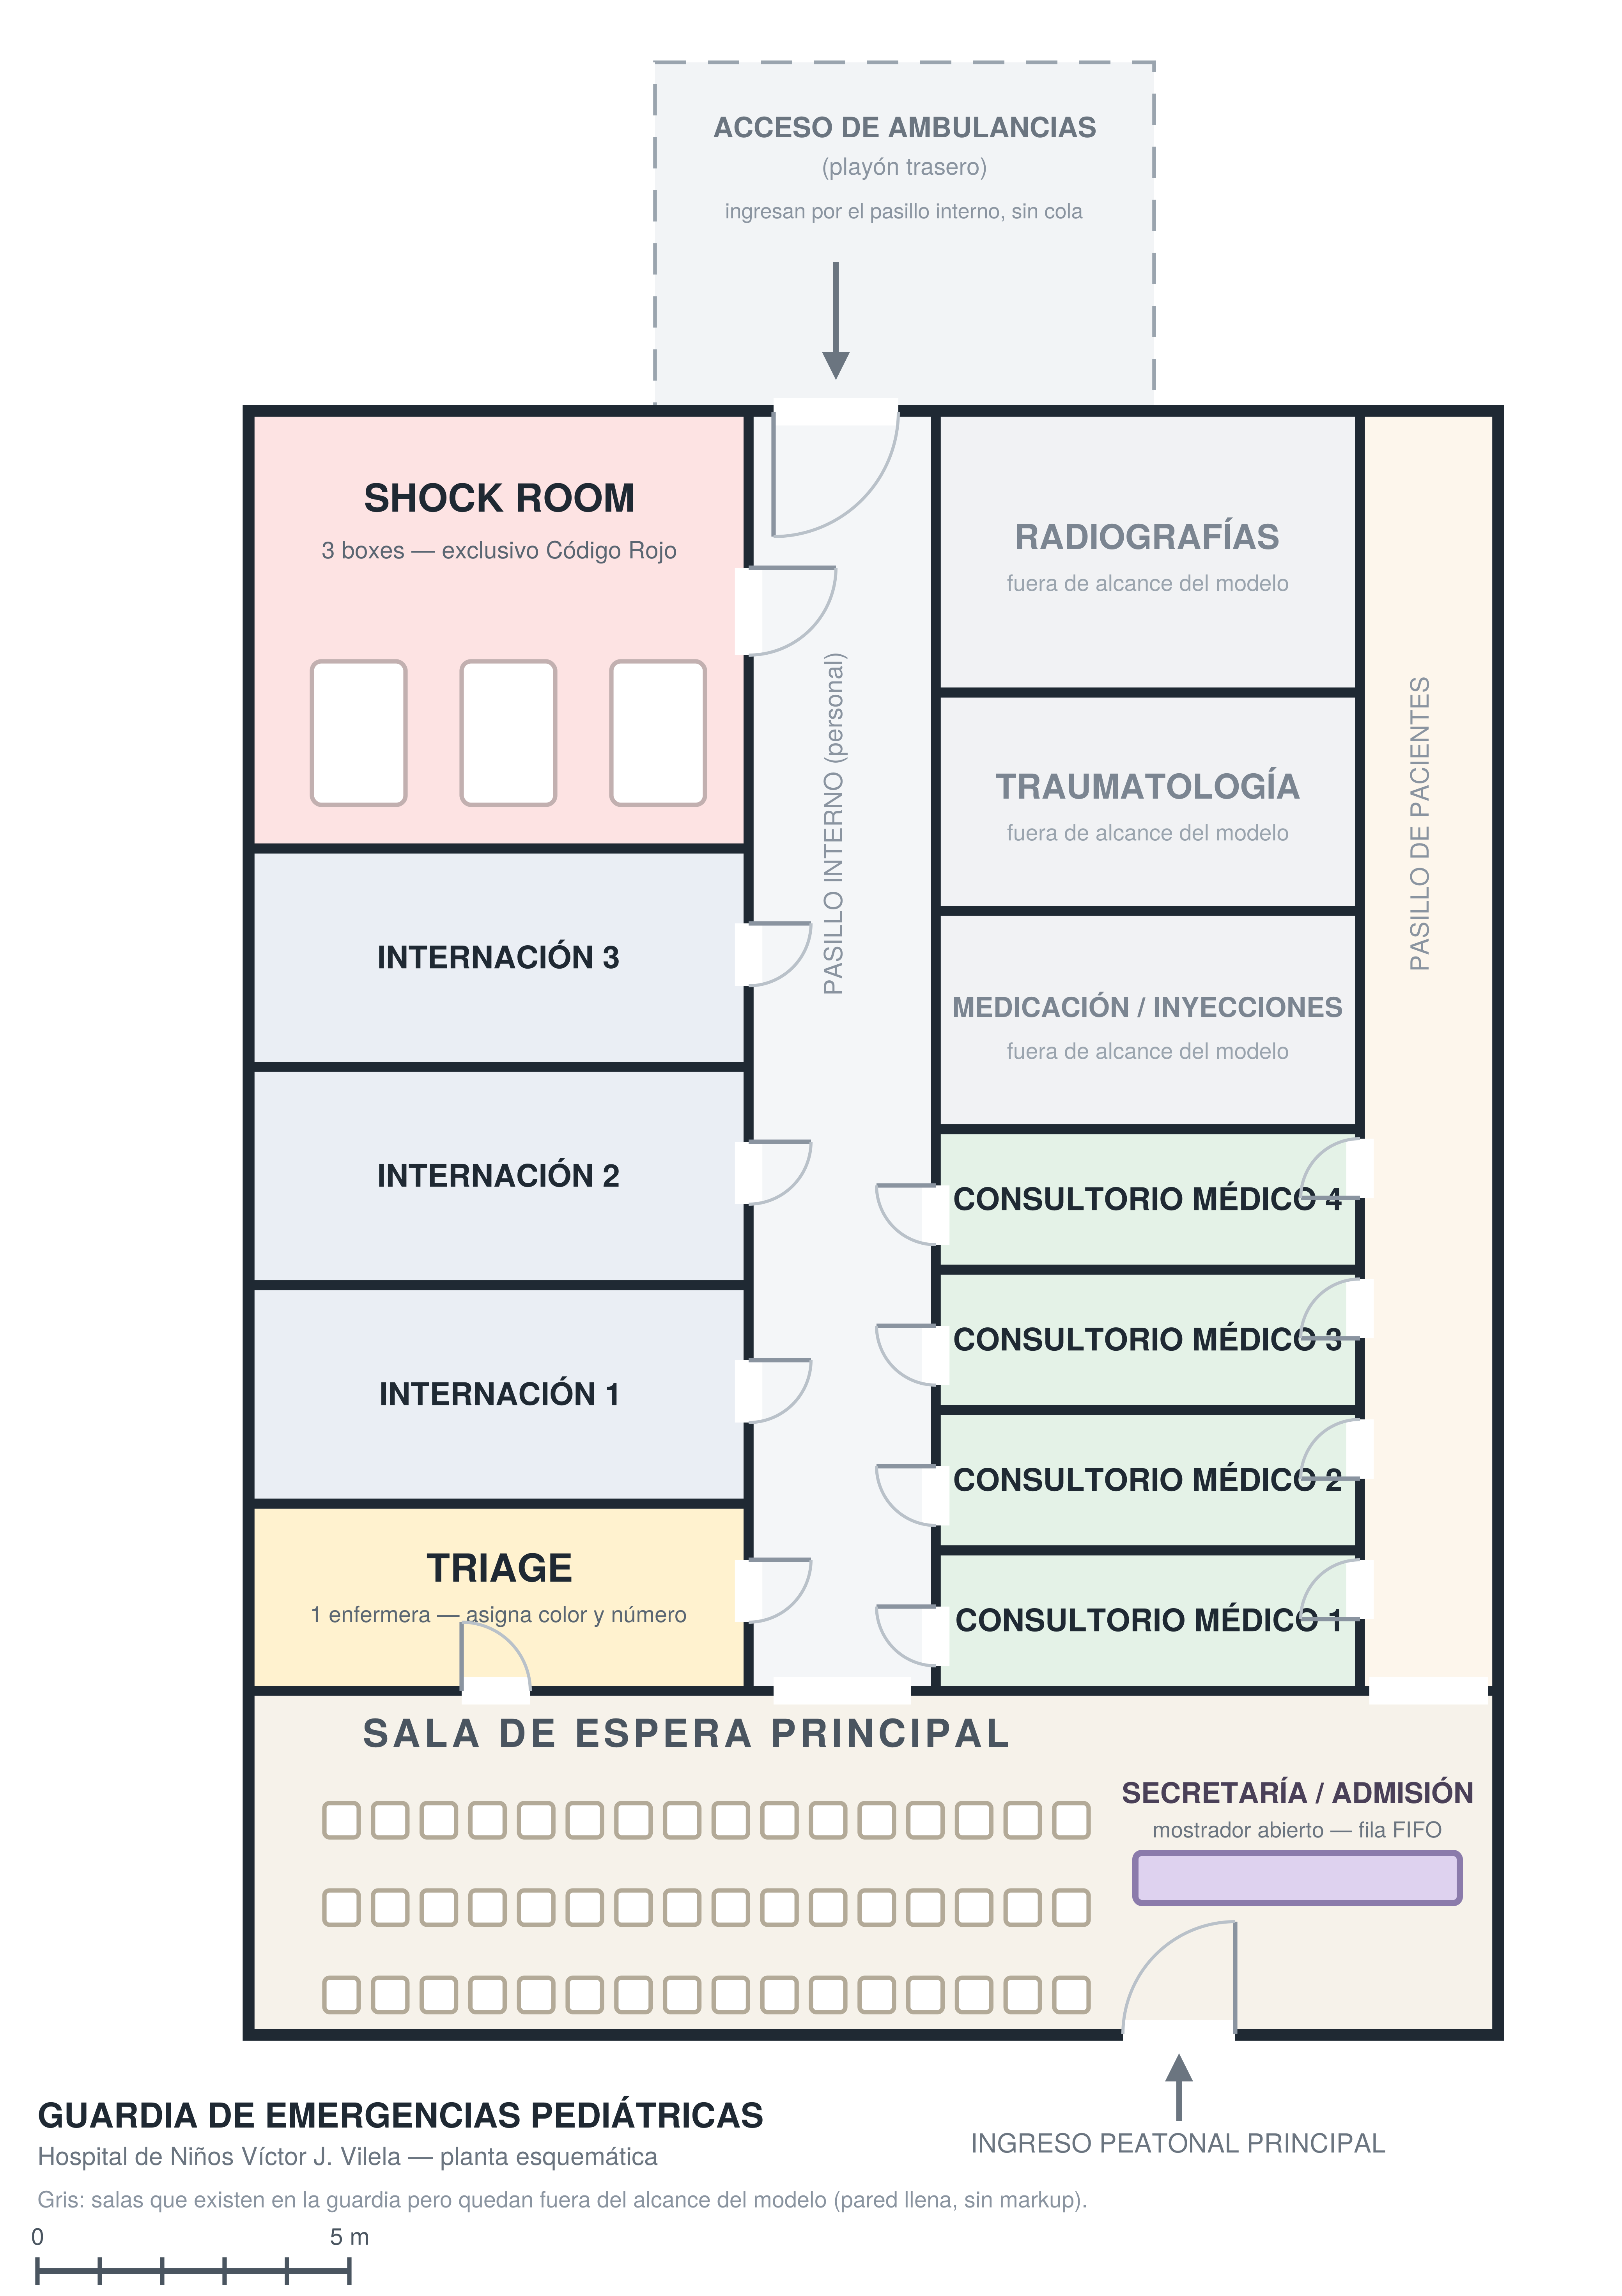
\includegraphics[width=0.85\textwidth]{plano_guardia_vilela.png}
  \caption{Plano de la guardia utilizado como base del modelo. Los sectores
  de traumatología, radiografías y medicación se representan en gris por
  encontrarse fuera del alcance.}
  \label{fig:plano}
\end{figure}

El plano permite representar tanto el recorrido físico de los pacientes como
la ubicación de los distintos puntos de atención, y es el soporte sobre el
cual la Pedestrian Library de AnyLogic calcula los desplazamientos.

\subsection{Entidad y atributos del modelo}
\label{sec:entidad}

La entidad principal es el paciente pediátrico. Cada paciente lleva consigo
los atributos que determinan su comportamiento dentro del sistema:

\begin{table}[H]
\centering
\begin{tabular}{lll}
\toprule
\textbf{Atributo} & \textbf{Tipo} & \textbf{Significado} \\
\midrule
\texttt{colorReal}            & \texttt{ColorTriage} & Gravedad clínica real \\
\texttt{codigo}               & \texttt{ColorTriage} & Color asignado en el triage \\
\texttt{prioridad}            & \texttt{int}         & Prioridad en la cola, derivada de \texttt{codigo} \\
\texttt{porAmbulancia}        & \texttt{boolean}     & Forma de ingreso \\
\texttt{detectadoEnPuerta}    & \texttt{boolean}     & Rojo identificado en el acceso \\
\texttt{destino}              & \texttt{Destino}     & Alta o internación \\
\texttt{consultorioAsignado}  & \texttt{int}         & Consultorio en que fue atendido \\
\texttt{tLlegada}             & \texttt{double}      & Instante de arribo \\
\texttt{tEntraColaTriage}     & \texttt{double}      & Ingreso a la cola de triage \\
\texttt{tInicioTriage}        & \texttt{double}      & Comienzo de la clasificación \\
\texttt{tFinTriage}           & \texttt{double}      & Fin de la clasificación \\
\texttt{tEntraColaConsultorio}& \texttt{double}      & Ingreso a la cola de prioridad \\
\texttt{tInicioConsulta}      & \texttt{double}      & Comienzo de la atención médica \\
\texttt{tSalida}              & \texttt{double}      & Egreso del sistema \\
\texttt{cuentaParaMetrica}    & \texttt{boolean}     & Pertenencia a la ventana de medición \\
\bottomrule
\end{tabular}
\caption{Atributos del agente \texttt{Paciente}.}
\end{table}

La distinción entre \texttt{colorReal} y \texttt{codigo} es central en este
trabajo y se desarrolla en la sección~\ref{sec:error}.

\subsection{Recursos y servidores}

A partir del relevamiento se consideran los siguientes recursos:

\begin{table}[H]
\centering
\begin{tabular}{llc}
\toprule
\textbf{Recurso} & \textbf{Disciplina de la cola} & \textbf{Servidores} \\
\midrule
Secretaría / admisión   & FIFO                    & 2 \\
Triage                  & FIFO                    & 1 \\
Consultorios médicos    & Prioridad no expulsiva  & 4 \\
Shock Room              & FIFO                    & 3 equipos, 8 camas \\
\bottomrule
\end{tabular}
\caption{Configuración base de recursos.}
\label{tab:recursos}
\end{table}

En el Shock Room se distingue el espacio físico de la capacidad de atención:
el sector dispone de ocho camas, pero sólo tres pacientes pueden ser
atendidos simultáneamente por limitación de personal. Esta distinción se
implementa mediante una cola de capacidad ocho y un conjunto de recursos de
capacidad tres.

\subsection{Flujo de pacientes}

El paciente peatonal atraviesa las siguientes etapas:

\begin{center}
Ingreso $\rightarrow$ Secretaría $\rightarrow$ Sala de espera $\rightarrow$
Triage $\rightarrow$ Sala de espera $\rightarrow$ Consultorio $\rightarrow$
Alta / Internación
\end{center}

Corresponde notar que el paciente atraviesa la sala de espera dos veces: una
vez antes del triage, en cola FIFO, y otra después, en cola ordenada por
prioridad. Ambas colas comparten el mismo espacio físico, lo que resulta
relevante para la métrica de hacinamiento.

Una fracción de los pacientes peatonales presenta un cuadro crítico
identificable en el acceso. Estos casos se derivan directamente al Shock Room
sin pasar por secretaría ni triage, igual que los pacientes de ambulancia.

\subsection{Clasificación y prioridad de atención}

Durante el triage los pacientes se clasifican en cuatro categorías. La
distribución estimada para un día pico invernal y las prioridades asociadas
son:

\begin{table}[H]
\centering
\begin{tabular}{lcc}
\toprule
\textbf{Código} & \textbf{Proporción} & \textbf{Prioridad} \\
\midrule
Rojo     & 1,0 \%  & 4 \\
Naranja  & 7,2 \%  & 3 \\
Amarillo & 25,5 \% & 2 \\
Verde    & 66,3 \% & 1 \\
\bottomrule
\end{tabular}
\caption{Distribución de gravedad real y prioridad de atención.}
\label{tab:colores}
\end{table}

\begin{pendiente}
El documento de avance anterior consignaba una proporción de pacientes rojos
del 3~\%, mientras que el modelo implementa 1~\%. Debe unificarse el valor y
dejar constancia del criterio adoptado.
\end{pendiente}

\subsection{Proceso de llegada}
\label{sec:arribos}

El Hospital Vilela registra aproximadamente 97.000 consultas anuales por
guardia, lo que equivale a unos 266 pacientes diarios. Distribuidos de manera
uniforme a lo largo de las 24 horas representarían alrededor de 11 pacientes
por hora.

El modelo implementado utiliza una tasa constante de \textbf{10 pacientes por
hora} para el ingreso peatonal y \textbf{0,2 por hora} para el ingreso en
ambulancia, sobre una ventana de ocho horas correspondiente al turno
vespertino. Este valor fue consultado con una profesional que se desempeña en
la guardia, quien lo consideró razonable para el día modelado.

Los arribos se modelan mediante un proceso de Poisson, que constituye el
supuesto estándar para llegadas independientes a un servicio de urgencias.

\begin{pendiente}
El documento de avance anterior proponía una tasa \emph{variable por franja
horaria} (13, 16, 18, 20, 19 y 16 pacientes por hora entre las 14:00 y las
20:00, aproximadamente 102 pacientes en seis horas), mientras que el modelo
implementa una tasa constante de 10 por hora durante ocho horas,
aproximadamente 80 pacientes. Las dos definiciones son incompatibles y debe
elegirse una. Debe tenerse presente que con la capacidad actualmente
representada en el modelo, una tasa media de 17 pacientes por hora conduce a
una utilización de los consultorios superior a la unidad, es decir, a un
sistema que no alcanza régimen estacionario.
\end{pendiente}

\subsection{Tiempos de servicio}

Los tiempos de atención se modelan mediante distribuciones triangulares. Esta
elección responde a una indicación de la cátedra y a una razón metodológica:
la triangular se define con tres valores --- mínimo, moda y máximo --- que es
precisamente lo que una persona con experiencia en el servicio puede estimar
en ausencia de registros históricos, y además no produce valores negativos.

\begin{table}[H]
\centering
\begin{tabular}{lc}
\toprule
\textbf{Proceso} & \textbf{Distribución (minutos)} \\
\midrule
Secretaría                  & triangular(1,5;\ 2,5;\ 4) \\
Triage                      & triangular(3;\ 5;\ 8) \\
Consulta verde              & triangular(10;\ 15;\ 22) \\
Consulta amarilla           & triangular(18;\ 25;\ 35) \\
Consulta naranja y roja     & triangular(35;\ 42;\ 50) \\
Atención en Shock Room      & triangular(60;\ 90;\ 150) \\
\bottomrule
\end{tabular}
\caption{Distribuciones de los tiempos de servicio.}
\label{tab:tiempos}
\end{table}

Los valores modales son consistentes con el relevamiento previo. Los extremos
de las distribuciones se consideran supuestos del grupo y deben revisarse
durante la validación.

\subsection{Destinos finales}

Una vez finalizada la atención el modelo considera dos destinos posibles:

\begin{table}[H]
\centering
\begin{tabular}{lcc}
\toprule
\textbf{Código real} & \textbf{Internación} & \textbf{Alta} \\
\midrule
Rojo     & 100 \% & 0 \% \\
Naranja  & 60 \%  & 40 \% \\
Amarillo & 20 \%  & 80 \% \\
Verde    & 2 \%   & 98 \% \\
\bottomrule
\end{tabular}
\caption{Probabilidad de internación según gravedad real.}
\label{tab:destinos}
\end{table}

Para el código rojo la derivación a internación no se modela como una
probabilidad sino como una regla del servicio: todo paciente cuya gravedad
real es roja termina internado.

Es importante señalar que el destino depende de \texttt{colorReal} y no de
\texttt{codigo}. Un paciente mal clasificado espera más o menos de lo que le
corresponde, pero su cuadro clínico --- y por lo tanto su destino --- no se
modifica por el error de clasificación.

\begin{pendiente}
La probabilidad de internación del código naranja permanece abierta entre
60~\% y 85~\%. El modelo implementa 60~\%.
\end{pendiente}

\subsection{Modelado explícito del error de triage}
\label{sec:error}

El modelo distingue la gravedad clínica real del paciente del color que le
asigna la enfermera. Esa diferencia es exactamente el sobre-triage y el
sub-triage, y constituye el objeto central del estudio.

\begin{itemize}
  \item \texttt{colorReal} se sortea al momento del arribo según la
  distribución de la tabla~\ref{tab:colores}. Determina cuánto dura la
  consulta y si el paciente termina internado.
  \item \texttt{codigo} se obtiene al finalizar el triage aplicando una
  función de clasificación sobre \texttt{colorReal}. Determina la prioridad
  en la cola de acceso al consultorio.
\end{itemize}

Cuando ambos coinciden, la clasificación fue correcta. Cuando no, el paciente
espera un tiempo que no corresponde a su gravedad.

La función de clasificación desplaza el color un escalón en la escala de
urgencia con probabilidad $p_{sub}$ hacia abajo y $p_{sobre}$ hacia arriba:

\begin{lstlisting}
double u = uniform();
if (u < pSubtriage) {
    switch (real) {
        case ROJO:     return ColorTriage.NARANJA;
        case NARANJA:  return ColorTriage.AMARILLO;
        default:       return ColorTriage.VERDE;
    }
}
if (u < pSubtriage + pSobretriage) {
    switch (real) {
        case VERDE:    return ColorTriage.AMARILLO;
        case AMARILLO: return ColorTriage.NARANJA;
        default:       return ColorTriage.ROJO;
    }
}
return real;
\end{lstlisting}

Los valores adoptados son $p_{sub} = 0{,}12$ y $p_{sobre} = 0{,}08$.

Debe notarse que la tasa de error \emph{observada} resulta menor que la
nominal, porque los extremos de la escala no pueden desplazarse más allá de
sí mismos: un paciente verde no puede ser sub-triado ni un rojo
sobre-triado. Dado que el verde representa cerca de dos tercios de los
arribos, la proporción efectiva de sub-triage se ubica en torno al 4~\%.

\begin{pendiente}
Los valores de $p_{sub}$ y $p_{sobre}$ son estimaciones del grupo sin
respaldo documental. Deben declararse como supuestos o sustituirse por
valores relevados.
\end{pendiente}

\subsection{Variables de entrada y de salida}

Las principales variables de entrada son la tasa de llegada, la distribución
de pacientes por código, la cantidad de servidores de cada tipo, los tiempos
de servicio, las probabilidades de internación y las tasas de error de
clasificación.

Como variables de salida se registran el tiempo de espera para el triage, el
tiempo de espera para el consultorio --- global y segregado por código ---,
el tiempo total de permanencia, la cantidad promedio de pacientes en la sala
de espera, la utilización de los recursos y los recuentos de sub y
sobre-triage.

% =====================================================================
\section{Validación del modelo conceptual}

Antes de su implementación, el modelo conceptual fue contrastado con el
relevamiento realizado y con la estructura física de la guardia.

\subsection{Correspondencia con el sistema real}

El flujo descripto en la sección~2.4 fue verificado contra el circuito que
sigue efectivamente un paciente en la guardia: ingreso por la puerta
principal, admisión administrativa, espera en la sala común, llamado a
triage, retorno a la sala, llamado a consultorio y egreso. La derivación
directa de los pacientes de ambulancia al Shock Room y la identificación de
casos críticos en el acceso también fueron confirmadas durante el
relevamiento.

\subsection{Decisiones de abstracción y su justificación}

\begin{itemize}
  \item \textbf{Espera en sala común.} Las dos colas del sistema --- triage y
  consultorio --- comparten un mismo espacio físico. El modelo conceptual las
  representa como colas lógicas separadas sobre una misma localización, lo
  que permite medir el hacinamiento agregado sin perder la distinción entre
  ambas esperas.
  \item \textbf{Prioridad no expulsiva.} Un paciente que ya comenzó su
  atención no es interrumpido por la llegada de otro más grave. Esta decisión
  refleja la práctica del servicio.
  \item \textbf{Internación como punto de salida.} Los procesos internos de
  las salas de internación no influyen sobre las métricas de interés, por lo
  que su exclusión no compromete la validez del modelo respecto del problema
  planteado.
  \item \textbf{Cola ciega previa al triage.} El modelo representa
  explícitamente que la priorización sólo existe aguas abajo de la
  clasificación, lo que resulta esencial para interpretar correctamente el
  escenario alternativo.
\end{itemize}

\subsection{Limitaciones conocidas del modelo conceptual}

\begin{itemize}
  \item No se modela el abandono de pacientes que se retiran sin ser
  atendidos. De existir en el sistema real, el modelo sobreestima la carga.
  \item No se modela la reclasificación de pacientes que empeoran durante la
  espera.
  \item La tasa de error de clasificación es independiente de la carga de
  trabajo.
  \item La exclusión de traumatología, radiografías y medicación concentra en
  cuatro consultorios una demanda que en el sistema real se reparte entre más
  sectores.
\end{itemize}

% =====================================================================
\section{Construcción y verificación del programa}

\subsection{Herramientas y bibliotecas empleadas}

El modelo fue implementado en AnyLogic 8.9.10 (Personal Learning Edition)
combinando dos bibliotecas:

\begin{itemize}
  \item La \textbf{Pedestrian Library}, que representa el desplazamiento
  físico de los pacientes sobre el plano de la guardia, incluyendo la
  ocupación del espacio en la sala de espera.
  \item La \textbf{Process Modeling Library}, que aporta las colas, los
  conjuntos de recursos y las demoras necesarias para representar la
  disciplina de atención.
\end{itemize}

La combinación de ambas responde a una necesidad concreta: la Pedestrian
Library no dispone de colas con prioridad, mientras que la Process Modeling
Library no desplaza peatones por el espacio.

\subsection{Estructura de bloques}

El modelo se organiza en cuatro cadenas:

\begin{table}[H]
\centering
\small
\begin{tabular}{ll}
\toprule
\textbf{Cadena} & \textbf{Secuencia de bloques} \\
\midrule
Ingreso peatonal &
  \texttt{pedSourcePeatonal} $\rightarrow$ \texttt{pedSelectRojoPuerta}
  $\rightarrow$ \texttt{pedServiceSecretaria} \\
Triage &
  \texttt{pedGoToSalaEspera} $\rightarrow$ \texttt{queueTriage} $\rightarrow$
  \texttt{seizeTriage} $\rightarrow$ \texttt{pedGoToTriage} \\
 & $\rightarrow$ \texttt{delayTriage} $\rightarrow$ \texttt{releaseTriage} \\
Consultorios &
  \texttt{queuePrioridad} $\rightarrow$ \texttt{seizeConsultorio} $\rightarrow$
  \texttt{pedGoToConsultorio} \\
 & $\rightarrow$ \texttt{delayConsulta} $\rightarrow$ \texttt{releaseConsultorio} \\
Shock Room &
  \texttt{pedGoToShockRoom} $\rightarrow$ \texttt{queueShock} $\rightarrow$
  \texttt{seizeShock} \\
 & $\rightarrow$ \texttt{delayShock} $\rightarrow$ \texttt{releaseShock} \\
\bottomrule
\end{tabular}
\caption{Organización de la lógica del modelo en AnyLogic.}
\end{table}

La enfermera de triage se modela como un conjunto de recursos
(\texttt{ResourcePool}) y no como un servicio con área propia. Esta decisión
es deliberada: permite que la espera se produzca en la sala común y no dentro
del consultorio de triage, lo que resulta indispensable para medir
correctamente el hacinamiento.

\subsection{Escala temporal}
\label{sec:escala}

La licencia Personal Learning Edition de AnyLogic limita las simulaciones que
emplean la Pedestrian Library a cinco horas de tiempo simulado. Dado que el
turno que se desea representar abarca ocho horas, se introdujo un factor de
escala temporal

\[
k = \frac{480 \text{ min reales}}{300 \text{ min simulados}} = 1{,}6
\]

implementado como un parámetro del modelo. Todos los tiempos de servicio se
dividen por $k$, todas las tasas de arribo se multiplican por $k$, y la
velocidad de desplazamiento de los peatones se multiplica por $k$. Los
diámetros de los peatones y las dimensiones del plano no se modifican, por
tratarse de magnitudes espaciales.

Esta transformación preserva exactamente el comportamiento del sistema de
colas. En efecto, la utilización de un recurso con $c$ servidores

\[
\rho = \frac{\lambda\, E[S]}{c}
\]

permanece invariante, puesto que $\lambda \to k\lambda$ y
$E[S] \to E[S]/k$. Por la ley de Little, $L = \lambda W$, las longitudes de
cola también se conservan. Los tiempos medidos, en cambio, resultan en
minutos simulados y se reconvierten multiplicando por $k$.

\subsection{Verificación del programa}

La verificación se realizó de manera incremental, ejecutando el modelo tras
cada incorporación y resolviendo los errores detectados antes de continuar.
Se documentan a continuación los principales defectos encontrados y
corregidos, por constituir evidencia del proceso de verificación.

\begin{table}[H]
\centering
\small
\begin{tabular}{p{5.4cm}p{8.4cm}}
\toprule
\textbf{Defecto detectado} & \textbf{Corrección aplicada} \\
\midrule
Pacientes detenidos sobre las líneas de destino &
Los bloques \texttt{Delay} no desplazan peatones. Se antepuso un
\texttt{PedGoTo} hacia el área correspondiente. \\
Espera de triage producida dentro del consultorio &
Se reemplazó el servicio con área propia por un \texttt{ResourcePool} con
espera en la sala común. \\
Pacientes sin destino asignado al llegar al bloque de derivación &
La asignación se trasladó del \texttt{On exit} al \texttt{On enter} del
bloque de demora, de modo que el valor quede definido antes de la evaluación
de la condición. \\
Discrepancia entre la salida elegida y la salida efectiva &
Para condiciones que se asignan en el mismo evento en que el peatón se
desplaza se activó la opción \emph{Choice is stochastic or volatile}. \\
Pacientes de ambulancia sin gravedad real asignada &
Se incorporó la asignación explícita en el bloque de origen. \\
Rama de internación sin conexión &
Se corrigió el enlace del puerto correspondiente. \\
\bottomrule
\end{tabular}
\caption{Defectos detectados durante la verificación y sus correcciones.}
\end{table}

Las pruebas de verificación aplicadas fueron:

\begin{enumerate}
  \item \textbf{Conservación de entidades.} La cantidad de pacientes
  ingresados debe igualar la suma de los egresados y los presentes en el
  sistema al cierre.
  \item \textbf{Consistencia de las distribuciones de entrada.} La proporción
  de colores observada debe aproximarse a la teórica de la
  tabla~\ref{tab:colores}.
  \item \textbf{Consistencia de los tiempos de servicio.} La media observada
  de cada servicio debe aproximarse a la media de su triangular.
  \item \textbf{Ausencia de bloqueos.} Ningún paciente debe permanecer
  inmóvil sobre una línea de destino durante la corrida.
  \item \textbf{Coherencia de la disciplina de prioridad.} La espera media de
  los pacientes verdes debe superar a la de los naranjas.
\end{enumerate}

% =====================================================================
\section{Ejecuciones piloto}
\label{sec:piloto}

Se realizaron ejecuciones piloto con la configuración base con el objeto de
detectar comportamientos anómalos antes de las corridas de producción.

\subsection{Utilización observada}

\begin{table}[H]
\centering
\begin{tabular}{lccc}
\toprule
\textbf{Recurso} & \textbf{Servidores} & \textbf{$\rho$ analítico} & \textbf{$\rho$ observado} \\
\midrule
Triage       & 1 & 0,88 & 0,958 \\
Consultorios & 4 & 0,84 & 0,939 \\
\bottomrule
\end{tabular}
\caption{Utilización analítica y observada en las ejecuciones piloto.}
\label{tab:piloto}
\end{table}

\subsection{Hallazgo principal}

Las ejecuciones piloto revelaron que el sistema no alcanza régimen
estacionario dentro del horizonte considerado. Al cierre de la corrida se
contabilizaron \textbf{55 pacientes en espera de consultorio} frente a
\textbf{5 en espera de triage}, sobre un total aproximado de 72 pacientes
arribados.

Dos conclusiones se desprenden de esta observación:

\begin{enumerate}
  \item \textbf{La restricción dominante son los consultorios médicos}, no el
  puesto de triage. La cola se acumula aguas abajo de la clasificación.
  \item \textbf{La magnitud de la acumulación excede lo esperable} para una
  utilización de 0,84. Un sistema M/M/4 con esa carga presenta una longitud
  media de cola del orden de tres a cinco pacientes, no de cincuenta y cinco.
\end{enumerate}

\begin{pendiente}
El segundo punto indica que el modelo todavía contiene un desajuste no
resuelto. La hipótesis principal, ya señalada en la sección~1.4, es que la
exclusión de traumatología, radiografías y medicación concentra en cuatro
consultorios una demanda que el sistema real reparte entre más sectores. Esta
sección debe completarse una vez resuelto el punto, incorporando los valores
definitivos de la tabla~\ref{tab:piloto}.
\end{pendiente}

\subsection{Sesgo de truncamiento}

Las ejecuciones piloto pusieron de manifiesto un problema metodológico
relevante. Las métricas de espera se registraban en el momento del egreso del
paciente, de modo que los pacientes que permanecían en cola al finalizar la
corrida no quedaban contabilizados.

En un sistema congestionado, los pacientes que alcanzan a egresar son
precisamente aquellos que esperaron menos, lo que introduce un sesgo
sistemático hacia valores bajos. El sesgo es además de magnitud distinta
entre escenarios, lo que invalida la comparación: cuanto más congestionado el
escenario, mayor la proporción de pacientes truncados y menor el promedio
observado.

La corrección aplicada consiste en registrar los tiempos de espera en el
instante en que comienza la atención y no en el egreso, de modo que todo
paciente que llegó a ser atendido quede contabilizado con independencia de si
completó su recorrido dentro del horizonte. Adicionalmente se registra el
número de observaciones de cada estadística como control de sanidad.

% =====================================================================
\section{Validación del modelo programado}

La validación del modelo programado se apoya en tres procedimientos
complementarios.

\subsection{Contraste con resultados analíticos}

Para las estaciones del sistema que admiten un tratamiento analítico se
comparó la utilización simulada con la calculada mediante teoría de colas.
Siendo $\lambda$ la tasa de arribos efectiva a la estación, $E[S]$ el tiempo
medio de servicio y $c$ el número de servidores:

\[
\rho = \frac{\lambda\, E[S]}{c}
\]

Para el puesto de triage, con $\lambda = 9{,}91$ pacientes por hora y
$E[S] = 5{,}33$ minutos, resulta $\rho = 0{,}88$. Para los consultorios, con
$E[S] = 20{,}3$ minutos ponderado por la distribución de colores y $c = 4$,
resulta $\rho = 0{,}84$.

La comparación de estos valores con los de la tabla~\ref{tab:piloto}
constituye la prueba de validación más exigente aplicada al modelo, por
cuanto un desvío significativo señala una inconsistencia en los parámetros o
en la estructura.

\subsection{Validación aparente}

El recorrido de los pacientes sobre el plano fue revisado visualmente durante
las corridas, verificando que la secuencia de desplazamientos se corresponda
con el circuito real: que la espera se produzca en la sala y no en los
consultorios, que los pacientes de ambulancia accedan directamente al Shock
Room y que los consultorios se ocupen de manera equilibrada.

\subsection{Validación con el sistema real}

\begin{pendiente}
Esta subsección debe completarse contrastando las salidas del modelo con el
conocimiento de la profesional del hospital consultada: ¿resultan
verosímiles los tiempos de espera obtenidos? ¿se corresponde la proporción de
internaciones con lo observado en la práctica? Se recomienda documentar esa
conversación como evidencia de validación.
\end{pendiente}

% =====================================================================
\section{Diseño de experimentos}

\subsection{Escenarios}

\begin{table}[H]
\centering
\begin{tabular}{llc}
\toprule
\textbf{Escenario} & \textbf{Descripción} & \textbf{Enfermeras de triage} \\
\midrule
Base        & Configuración actual del servicio & 1 \\
Alternativo & Segundo puesto de clasificación en paralelo & 2 \\
\bottomrule
\end{tabular}
\caption{Escenarios comparados.}
\end{table}

El escenario alternativo modifica un único parámetro del modelo. La
estructura, las distribuciones y el resto de los supuestos permanecen
idénticos, lo que garantiza que cualquier diferencia observada sea atribuible
al cambio de dotación.

La justificación de este escenario es doble. Por una parte, el triage es la
única estación del sistema con un servidor único, configuración que en teoría
de colas resulta especialmente sensible a la variabilidad. Por otra, la cola
previa al triage es una cola ciega: todo minuto de espera anterior a la
clasificación transcurre sin priorización, de modo que reducirla beneficia
desproporcionadamente a los pacientes cuya urgencia todavía no fue
reconocida. Se trata además de la intervención de menor costo que el servicio
podría evaluar, frente a la alternativa de habilitar un quinto consultorio.

\subsection{Hipótesis de trabajo}

Se espera que la incorporación del segundo puesto reduzca de manera clara la
espera hasta la clasificación. Sin embargo, la mejora en el tiempo total de
permanencia debería resultar menor que el tiempo de espera de triage
eliminado, por dos razones: en régimen, el caudal de pacientes que alcanza la
cola de consultorios lo determinan los arribos y no el triage; y la
eliminación del puesto saturado suprime un efecto regulador que espaciaba la
entrada a la segunda cola.

La pregunta que responde la simulación es, en consecuencia, si el cuello de
botella se resuelve o simplemente se traslada.

\subsection{Horizonte y ventana de medición}

\begin{table}[H]
\centering
\begin{tabular}{ll}
\toprule
\textbf{Aspecto} & \textbf{Definición} \\
\midrule
Horizonte de simulación       & 300 minutos simulados (480 minutos reales) \\
Factor de escala temporal     & $k = 1{,}6$ \\
Período de calentamiento      & 45 minutos reales, descartados \\
Ventana de medición           & Minutos reales 45 a 405 \\
Réplicas por escenario        & 30 \\
Generación de números aleatorios & Semilla aleatoria por réplica \\
\bottomrule
\end{tabular}
\caption{Parámetros del diseño experimental.}
\end{table}

El período de calentamiento descarta el arranque con la guardia vacía, que no
representa una condición real de operación. El cierre anticipado de la
ventana de medición evita que los pacientes que no alcanzan a completar su
recorrido distorsionen los promedios.

La elección de treinta réplicas responde a la necesidad de disponer de una
muestra suficiente para estimar intervalos de confianza y aplicar el test de
medias. Con una única corrida por escenario la variabilidad entre réplicas
de una misma configuración puede superar la diferencia entre configuraciones,
de modo que ninguna conclusión sería sostenible.

\subsection{Variables de respuesta}

\begin{table}[H]
\centering
\small
\begin{tabular}{llp{6.2cm}}
\toprule
\textbf{Indicador} & \textbf{Unidad} & \textbf{Fundamento} \\
\midrule
Espera hasta el triage & min & Mide la cola ciega, sin priorización. \\
Espera hasta el consultorio & min & Detecta el traslado del cuello de botella. \\
Espera de pacientes verdes & min & Métrica~1 comprometida. \\
Espera de urgencias reales & min & Métrica adicional comprometida. \\
Permanencia total & min & Efecto neto sobre el paciente. \\
Pacientes en sala de espera & pacientes & Métrica~2, hacinamiento físico. \\
Utilización de los recursos & --- & Verificación y diagnóstico. \\
Recuento de sub y sobre-triage & pacientes & Calidad de la clasificación. \\
\bottomrule
\end{tabular}
\caption{Indicadores medidos y su justificación.}
\end{table}

La separación entre la espera de triage y la espera de consultorio resulta
esencial: si se midiera únicamente el tiempo total, un traslado del cuello de
botella sería indistinguible de la ausencia de efecto.

% =====================================================================
\section{Corridas de producción}

Las corridas de producción se ejecutan mediante un experimento de variación
de parámetros sobre el número de enfermeras de triage, con treinta réplicas
independientes por nivel, totalizando sesenta corridas.

\begin{pendiente}
Esta sección debe completarse una vez resuelto el desajuste señalado en la
sección~\ref{sec:piloto}. Debe documentarse el número de corridas efectuadas,
el tiempo de cómputo requerido y cualquier incidencia observada durante la
ejecución.
\end{pendiente}

% =====================================================================
\section{Análisis de los datos de salida}

\subsection{Resultados por escenario}

\begin{table}[H]
\centering
\small
\begin{tabular}{lcccc}
\toprule
 & \multicolumn{2}{c}{\textbf{Escenario base}} & \multicolumn{2}{c}{\textbf{Escenario alternativo}} \\
\cmidrule(lr){2-3}\cmidrule(lr){4-5}
\textbf{Indicador} & \textbf{Media} & \textbf{Desvío} & \textbf{Media} & \textbf{Desvío} \\
\midrule
Espera hasta el triage      & --- & --- & --- & --- \\
Espera hasta el consultorio & --- & --- & --- & --- \\
Espera de pacientes verdes  & --- & --- & --- & --- \\
Espera de urgencias reales  & --- & --- & --- & --- \\
Permanencia total           & --- & --- & --- & --- \\
Pacientes en sala de espera & --- & --- & --- & --- \\
\bottomrule
\end{tabular}
\caption{Resultados sobre 30 réplicas por escenario.}
\label{tab:resultados}
\end{table}

\subsection{Test de medias}

Para determinar si las diferencias observadas entre escenarios resultan
estadísticamente significativas se aplica un test de diferencia de medias
para muestras independientes. Las réplicas de cada escenario se generan con
semillas distintas e independientes entre sí, por lo que las dos muestras son
independientes. No se asume igualdad de varianzas, de modo que se emplea el
test de Welch.

Sean $\bar{x}_1$ y $\bar{x}_2$ las medias muestrales de cada escenario,
$s_1^2$ y $s_2^2$ sus varianzas muestrales y $n_1 = n_2 = 30$ el número de
réplicas. Las hipótesis son

\[
H_0: \mu_1 = \mu_2
\qquad\text{frente a}\qquad
H_1: \mu_1 \neq \mu_2
\]

con un nivel de significancia $\alpha = 0{,}05$.

El estadístico de contraste es

\begin{equation}
t = \frac{\bar{x}_1 - \bar{x}_2}
         {\sqrt{\dfrac{s_1^2}{n_1} + \dfrac{s_2^2}{n_2}}}
\label{eq:t}
\end{equation}

y los grados de libertad se aproximan mediante la ecuación de
Welch--Satterthwaite:

\begin{equation}
\nu = \frac{\left(\dfrac{s_1^2}{n_1} + \dfrac{s_2^2}{n_2}\right)^{\!2}}
           {\dfrac{\left(s_1^2/n_1\right)^2}{n_1 - 1} +
            \dfrac{\left(s_2^2/n_2\right)^2}{n_2 - 1}}
\label{eq:welch}
\end{equation}

Se rechaza $H_0$ cuando $|t| > t_{\nu,\,1-\alpha/2}$.

El intervalo de confianza del $100(1-\alpha)\%$ para la diferencia de medias
resulta

\begin{equation}
(\bar{x}_1 - \bar{x}_2) \;\pm\;
t_{\nu,\,1-\alpha/2}\,
\sqrt{\frac{s_1^2}{n_1} + \frac{s_2^2}{n_2}}
\label{eq:ic}
\end{equation}

El intervalo de confianza resulta más informativo que el valor $p$ para los
fines de este trabajo, por cuanto expresa la magnitud de la mejora en las
mismas unidades del indicador y permite juzgar su relevancia operativa, y no
solamente su significancia estadística.

\begin{table}[H]
\centering
\small
\begin{tabular}{lccccc}
\toprule
\textbf{Indicador} & \textbf{Diferencia} & $t$ & $\nu$ & \textbf{IC 95\%} & \textbf{Decisión} \\
\midrule
Espera hasta el triage      & --- & --- & --- & --- & --- \\
Espera hasta el consultorio & --- & --- & --- & --- & --- \\
Espera de pacientes verdes  & --- & --- & --- & --- & --- \\
Espera de urgencias reales  & --- & --- & --- & --- & --- \\
Permanencia total           & --- & --- & --- & --- & --- \\
Pacientes en sala de espera & --- & --- & --- & --- & --- \\
\bottomrule
\end{tabular}
\caption{Test de medias entre escenarios. Nivel de significancia 0,05.}
\label{tab:test}
\end{table}

\begin{pendiente}
Completar las tablas~\ref{tab:resultados} y~\ref{tab:test} con los resultados
de las corridas de producción. Las fórmulas~\eqref{eq:t},
\eqref{eq:welch} y~\eqref{eq:ic} se aplican sobre las sesenta observaciones
exportadas desde AnyLogic.
\end{pendiente}

\subsection{Interpretación}

El diseño del estudio permite distinguir tres desenlaces posibles, cada uno
con una recomendación distinta:

\begin{table}[H]
\centering
\small
\begin{tabular}{p{3.6cm}p{5.0cm}p{5.0cm}}
\toprule
\textbf{Desenlace} & \textbf{Evidencia que lo identifica} & \textbf{Implicancia} \\
\midrule
El cuello de botella se resuelve &
Cae la espera de triage y la permanencia total disminuye en magnitud
comparable. La espera de consultorio aumenta poco. &
El triage era la restricción efectiva. La incorporación se justifica por sí
sola. \\
El cuello de botella se traslada &
Cae la espera de triage pero la de consultorio aumenta en magnitud similar.
La permanencia total apenas se modifica. &
La restricción son los consultorios. La medida mejora la oportunidad de la
clasificación, no la congestión. \\
El sistema se satura aguas abajo &
La cola de consultorios crece de manera sostenida durante toda la ventana de
medición. &
La capacidad médica es insuficiente para el caudal. Corresponde evaluar un
quinto consultorio. \\
\bottomrule
\end{tabular}
\caption{Desenlaces posibles del estudio y su interpretación.}
\end{table}

Cabe destacar que incluso en el segundo desenlace la intervención conserva
valor clínico, puesto que desplaza la espera desde una cola ciega hacia una
cola priorizada: el paciente grave espera menos aunque el promedio del
conjunto se modifique poco. La ausencia de diferencia significativa en el
tiempo total constituye, en ese caso, un resultado válido y relevante.

% =====================================================================
\section{Documentación, conclusiones y recomendaciones}

\subsection{Conclusiones}

\begin{pendiente}
Completar con las conclusiones derivadas de los resultados obtenidos. Deben
responder explícitamente a la pregunta de decisión formulada en la
sección~1.2 y vincularse con los tres desenlaces previstos.
\end{pendiente}

\subsection{Recomendaciones}

\begin{pendiente}
Formular las recomendaciones dirigidas al servicio, distinguiendo entre
aquellas que el modelo respalda con evidencia estadística y aquellas que
constituyen sugerencias de prudencia.
\end{pendiente}

\subsection{Limitaciones del estudio}

\begin{itemize}
  \item \textbf{Origen de los datos.} Con excepción de la tasa de arribos,
  consultada con una profesional del servicio, los valores numéricos son
  estimaciones del grupo y no provienen de registros del hospital. Los
  tiempos de servicio, las probabilidades de internación y las tasas de error
  de clasificación constituyen supuestos.
  \item \textbf{Horizonte de simulación.} La licencia educativa limita las
  corridas con Pedestrian Library a cinco horas de tiempo simulado, lo que
  obligó a introducir el factor de escala descripto en la
  sección~\ref{sec:escala}.
  \item \textbf{Velocidad de desplazamiento.} El escalado temporal exige
  multiplicar la velocidad de los peatones por el mismo factor, lo que
  distorsiona levemente la dinámica de los cuellos de botella físicos. Dado
  que los desplazamientos representan segundos frente a esperas de decenas de
  minutos, el efecto sobre las métricas se considera despreciable.
  \item \textbf{Alcance.} La exclusión de traumatología, radiografías y
  medicación concentra en los consultorios generales una demanda que el
  sistema real reparte.
  \item \textbf{Ausencia de abandonos.} El modelo no representa a los
  pacientes que se retiran sin ser atendidos.
  \item \textbf{Régimen estacionario.} Con utilizaciones cercanas a la unidad
  y un horizonte acotado, el sistema puede no alcanzar régimen estacionario,
  de modo que los promedios dependen de la duración de la corrida.
\end{itemize}

\subsection{Trabajo futuro}

\begin{itemize}
  \item Incorporar un segundo escenario alternativo consistente en la
  derivación de pacientes verdes a centros de atención primaria.
  \item Hacer depender la probabilidad de error de clasificación de la carga
  de trabajo del puesto de triage, de modo que el escenario alternativo
  incida también sobre la calidad de la clasificación y no sólo sobre los
  tiempos.
  \item Sustituir la tasa de arribos constante por una tasa variable por
  franja horaria.
  \item Incorporar el abandono de pacientes en espera.
  \item Validar los tiempos de servicio y las probabilidades de internación
  contra registros del hospital.
\end{itemize}

\subsection{Datos que permitirían refinar el modelo}

En caso de obtenerse acceso a registros del servicio, los datos de mayor
valor para el estudio serían los siguientes, ordenados por impacto:

\begin{enumerate}
  \item Marcas de tiempo de arribo de cada paciente, sobre varias semanas, que
  permitirían verificar el supuesto de tasa constante y estimar la variación
  horaria.
  \item Duración registrada del triage y de la consulta médica, discriminada
  por color.
  \item Proporción de pacientes derivados a traumatología, radiografías y
  medicación, que determinaría el caudal efectivo hacia los consultorios
  generales.
  \item Destino final por color, que permitiría cerrar la discusión sobre la
  probabilidad de internación del código naranja.
  \item Proporción de pacientes que se retiran sin ser atendidos.
\end{enumerate}

Debe señalarse que ninguno de estos datos requiere identificación de
pacientes: marcas de tiempo, color, consultorio y destino son suficientes, lo
que facilita su obtención desde el punto de vista del resguardo de la
información personal.


\begin{thebibliography}{9}

\bibitem{ross}
Ross, S. M.
\textit{Simulation}.
Academic Press.

\bibitem{lawkelton}
Law, A. M. y Kelton, W. D.
\textit{Simulation Modeling and Analysis}.
McGraw-Hill.

\bibitem{anylogic}
AnyLogic.
\textit{AnyLogic Help: Pedestrian Library}.
\url{https://anylogic.help/library-reference-guides/pedestrian-library/index.html}

\end{thebibliography}

\begin{pendiente}
Verificar edición y año de cada referencia contra los ejemplares utilizados
en la cátedra, y agregar la bibliografía específica sobre triage pediátrico
que respalde la clasificación en cuatro niveles. El enunciado no admite
Wikipedia como referencia.
\end{pendiente}

\end{document}
